\chapter{INTRODUCTION TO THE STANDARD MODEL}\label{Ch1}

The Particle Physics is probing the smallest objects that are known as elementary particles and tries to extend our knowledge of the subatomic world. These elementary particles are accelerated, collided and detected at very high energies in the experiments around the globe - one of them being the largest experimental setup ever built for science - and studied after being detected. The Standard Model of particle physics (SM) is the theory of the fundamental interactions in this pursuit. It is a quantum field theory developed with the contribution of many scientists around the globe mainly in the second half of the 20$^{th}$ century and, over the last few decades, it has been shown to be an accurate description of the picture. It describes all known particles but is a mathematical description of three of the four known fundamental forces of the nature. These are the electromagnetic interaction, the weak and the strong nuclear interactions. The gravitational force, due to difficulties in combining general relativity with quantum mechanics, does not take place in the Standard Model. The gravity is known to be 10$^{40}$ times weaker than the electromagnetic force, thus its effects are expected to be negligible in the theory.

In the SM, the elementary particles of matter and the ones that carry forces between them is grouped into two, namely fermions and bosons. The distinction shows itself in their spin properties; fermions have a spin value of half an integer whereas the bosons have integer spin values. Besides, the fermions obey the Pauli exclusion principle meaning that they cannot be at the same quantum state, whereas the bosons do not obey the same rule. The first generation of fermions include up and down quarks, electron and its neutrino pair; and bosons include photons, W and Z bosons, gluons and the Higgs boson. When added the second and the third generation of particles - whose existence is one of the mysteries of nature - along with their anti-particles, they form the fundamental particles that are known today. A tabular form of these particles can be seen in~\autoref{SM-figure}.

\vspace{6pt}
\begin{figure}[ht]
	\centering
	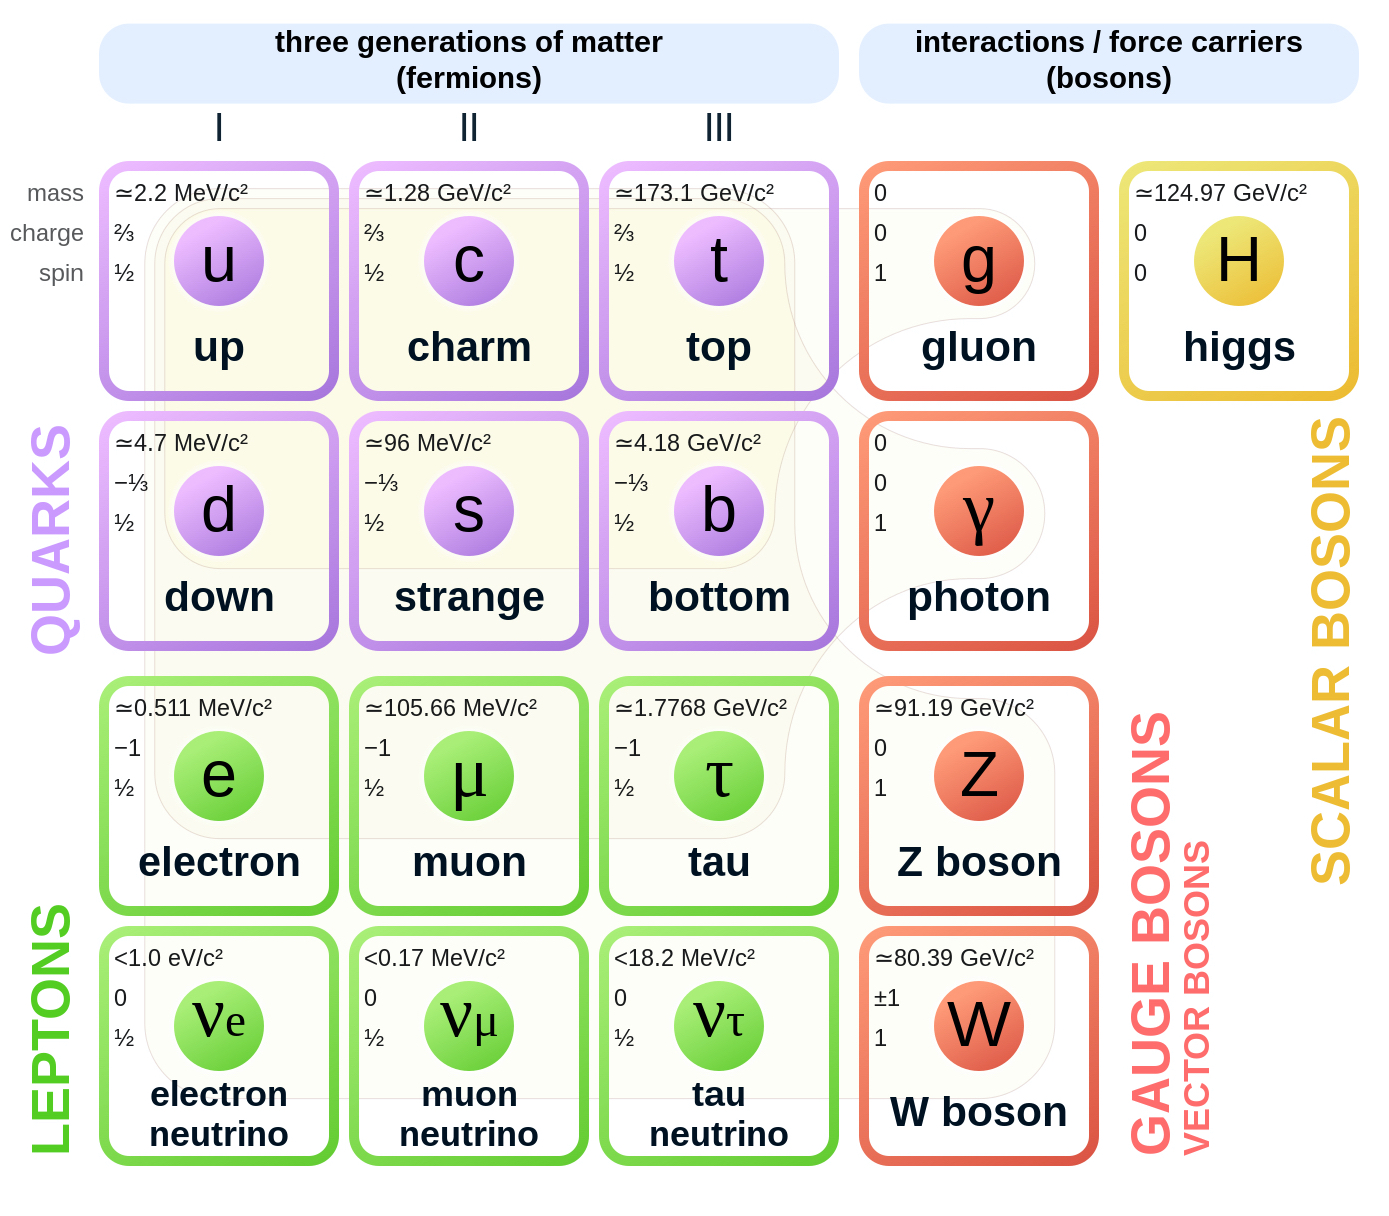
\includegraphics[width=\textwidth]{SM.jpg}
	\vspace{6pt}
	\caption{The elementary particles of the Standard Model. The fermions and bosons are grouped in columns where the quarks, leptons, gauge bosons and scalar Higgs boson are shown in different colours. The three generations of matter are indicated with roman numerals. The mass, charge and spin values corresponding to each particle are indicated on the upper left of each box. The bosons are shown in faint yellow areas with which they interact with.}
	\label{SM-figure}
\end{figure}

Fermions make up the ordinary matter that we see around us everyday. A subgroup of fermions are the leptons and they include electron, muon, tau and their neutrino pairs. Neutrinos have very small mass values compared to other leptons and quarks. They do not have electromagnetic charge which makes them obey only the weak force and they barely interact with matter. Flavours of leptons other than the neutrinos (electrons, muons and taus) have sizeable mass and charge and they are members of the three generations of matter.

The other type of leptons are the quarks. They have three generation as leptons do, and they include six different flavours, namely up, down, charm, strange, top and bottom quarks. They interact with electromagnetic, weak and strong nuclear forces since they have colour charges in addition to their electric charge. 

Bosons are the mediator particles of the three forces described in the SM. The particles of this type are called the gauge boson and they include the photon ($\gamma$), W$^{\pm}$ bosons, Z boson, gluons and the Higgs boson. The photons and gluons do not have mass where W bosons have about 80 GeV/c$^{2}$, Z boson has 91 GeV/c$^{2}$ and the Higgs boson has 125 GeV/c$^{2}$ of mass. Among these, only the W$^{\pm}$ bosons have electric charge, and only the Higgs boson has a spin value of zero making it a scalar boson where all other bosons are spin-1 gauge bosons, meaning that they are vector bosons.

The electromagnetic force, whose quantum field theory is established by the \emph{Quantum Electrodynamics (QED)}, is mediated by photons and acts only on the charged particles.  Almost everything we see in the daily life is thanks to the electromagnetic interactions. The carrier of this force, the photons, do not have the charge of the interaction type, hence do not self-interact. Since the photons have zero mass, their interaction range is unlimited.

The weak interaction, which is responsible for the decay of the particles that is a flavour changing interaction, acts only on the fermions. It has a very short interaction range. The neutral and the charged current interactions are mediated by the vector bosons of the this force, the Z boson and the W$^{\pm}$ bosons, respectively. The Higgs boson in this picture, plays the role of generating the masses of the W$^{\pm}$, and Z bosons through the Higgs mechanism~\cite{Higgs1964, BroutEnglert, Guralnik1964}, and of the quarks and leptons through the Yukawa interaction\cite{Weinberg1967}.

\emph{Quantum Chromodynamics (QCD)} is the theory of the strong interaction and describes the interaction between quarks mediated by the massless gluons. It has an interaction range of about $10^{-15}$ m. Unlike the electromagnetic interaction, the gauge bosons of the strong force possess the charge of the interaction, namely colours, hence can couple to itself. There are 3 types of colour; red, green and blue. Each quark in the universe carry one of these 3 colours - they carry anti-colour if they are anti-quarks - and gluons can be thought of colour carrier particles.

A phenomenon called \emph{the colour confinement} states that colour-charged particles cannot be isolated, meaning that only colour-neutral particles can be observed in nature\footnotemark. This results in that gluons carry a pair of charge consisting a colour and an anti-colour. Also, the hadrons are colour-neutral in two ways; i) with a pair of colour and anti-colour ii) with 3 different types of colour or anti-colour. The first combination makes up mesons, consisting of a quark pair (a quark and an anti-quark) and the second combination forms baryons.

\footnotetext{~Below the Hagedorn temperature ($T_H$) of about 0.15 GeV. At the energies higher than $1.7x10^{12}$ K, hadrons become unstable and it can be thought of the boiling point of the hadronic matter~\cite{Hagedorn2016}.}

Some of the predictions of the SM are observed in the experiments, and there is no other particle or force is found beyond the scope of the SM. However, the SM does not provide answers to the unsolved problems in the fundamental physics such as the non-zero masses of the neutrinos\cite{neutrino-mass}, or the dark matter and the dark energy\cite{PlanckCol} which are the dominated energy content of the universe. Therefore the SM is seen as an effective field theory.

\section{The Standard Model Lagrangian and the Higgs Mechanism}
\label{theSMandHiggs}

The Standard Model describes the mentioned fundamental interactions and elementary particles in a single Lagrangian. It is often considered in two parts: the strong sector offers a description for the particles with colour charges, while the electroweak part consists of the electromagnetism and the weak force. The SM is a renormalised gauge field theory with the $ SU(3)_C \otimes SU(2)_L \otimes U(1)_Y$ gauge form and the charges are colour, weak isospin and hypercharge, respectively. The SU(2)$_L$ and U(1)$_Y$ groups mix and the W$^{\pm}$, Z and $\gamma$ bosons are created where $SU(3)_C$ gauge group describes the strong force. The Lagrangian here, does not involve the particle masses but they are introduced to the theory via \emph{the spontaneous symmetry breaking} of the $SU(2)_L \otimes U(1)_Y$ group, that is the electroweak gauge group, which we will address after studying the SM Lagrangian.

Mathematical interpretation of the SM is provided by \emph{the Quantum Field Theory (QFT)}, where each particle is represented by a quantum field that is pervaded across the space-time. These fields are,
\begin{itemize}
  \item the fermion fields $\psi$,
  \item the electroweak boson fields $W_1$, $W_2$, $W_3$ and B,
  \item the gluon field $G_a$,
  \item the Higgs field $\phi$.
\end{itemize}

The behaviour of the the fundamental fields and the quantum states are determined by the Lagrangian density (usually called \emph{the Lagrangian}). Most of the field theories normally starts with defining a set of symmetries of the system and continues with writing down the renormalisable Lagrangian of the particles or fields that obey these symmetries. The QFT also follows this path; it consists of translational symmetry, rotational symmetry and a boost symmetry that is the invariance of an inertial reference frame. The internal symmetry that defines the SM is a local gauge symmetry of the $ SU(3) \otimes SU(2) \otimes U(1)$ group, where U(1) acts on B and $\phi$, SU(2) acts on W and $\phi$ and SU(3) acts on G fields. The fermion fields also, depending on their charge, transform under these symmetries. The Lagrangian of the SM can be interpreted in three parts; kinetic terms, coupling terms and the mass terms explained by the Higgs mechanism.

\subsection{Kinetic terms}

The kinetic terms, describing the motion of a particle, along with the mass term, represents a free particle. The kinetic term for a fermion field is given by
\be
i\bar\psi\gamma^\mu\psi ,
\ee
where $\gamma^\mu$ denotes the Dirac matrices. In order to find the kinetic terms for the gauge fields, we need to first define the field strength tensor for the spin-1 fields as,
\be
F_{\mu\nu}^a = \partial_\mu A_\nu^a-\partial_\nu A_\mu^a+g f^{abc}A_\mu^b A_\nu^c \hspace{1cm} a,b,c = 1,2,3 ,
\ee
for a given field A with coupling constant g and $f^{abc}$ being the structure constant of the prevailing gauge group defined by the commutator with generators $t_i$;
\be
[t_a,t_b]=if^{abc}t_c .
\ee
Here, we need to bring in three fields that correspond to SM gauge groups.
\begin{itemize}
    \item $B_{\mu}$; the gauge field for the U(1) of weak hypercharge with coupling constant $g\prime$ (or $g_1$) and gauge field tensor $B_{\mu\nu}$,
    \item $W_\mu^a$; the gauge field for the SU(2) group where \emph{a} runs over the three generators of this group. The coupling constant in denoted $g$ or $g_2$ and the gauge field tensor is represented by $W_{\mu\nu}^a$,
    \item $G_\mu^a$; the gluon field of SU(3) where \emph{a} runs over 8 colours. The coupling constant is denoted $g_s$ or $g_3$ and $G_{\mu\nu}^a$ is the gluon field tensor.
\end{itemize}
The kinetic term including all the gauge groups of the SM can be written as,
\be
\Lag_{kin} = -\frac{1}{4g_3^2}\sum_{A=1}^8 G_{\mu\nu}^A G^{\mu\nu A}-\frac{1}{4g_2^2} \sum_{a=1}^3 W_{\mu\nu}^a W^{\mu\nu a}-\frac{1}{4g_1^2} B_{\mu\nu} B^{\mu\nu} ,
\ee
where the structure constants of the U(1) gauge group  cancel out since the generators commute with each other, which is the general case for the Abelian groups. 

\subsection{Coupling terms}

Our approach in this section will be to "couple" the gauge fields to the fermions which leads to the interactions. We can interpret the coupling terms in two parts; the electroweak sector and the quantum chromodynamics sector.

The electroweak sector describes the interaction of the $SU(2)_L\otimes U(1)$ part of the Standard Model's gauge groups. The subscript L of the SU(2) group indicates that the field couples only to the left handed fermions. This is due to the parity-symmetry-violating nature of the weak interaction, which means that the $W^\pm$ bosons are only involved in charged-current interactions of left-handed particles and of right-handed antiparticles. However the $Z$ boson, carrying no electric charge, interacts with both right-handed and left-handed fermion states. In this sense, fermion fields are described with chirality components as left-handed doublets and right-handed singlets. The Lagrangian for the electroweak sector then becomes,
\be
\Lag_{EW} = \sum_\psi\bar\psi\gamma^\mu\left(i\partial_\mu -g_2\frac{1}{2}Y_WB_\mu-g\frac{1}{2}\sigma W_\mu\right)\psi
\ee
where $B_\mu$ and $W_\mu$ are the U(1) and SU(2) gauge fields as defined in \autoref{theSMandHiggs}, $Y_W$ is the weak hypercharge which is the generator of the U(1) gauge group and the components of the $\sigma$ are the Pauli matrices which are the generators of the SU(2) group with the eigenvalues that give the weak isospin values. Here the weak hypercharge symmetry of U(1) is defined different than the Quantum Electrodynamics (QED) in order to unify the electrodynamics with the weak interactions. The relation between the electric charge Q, and the hypercharge $Y_W$ is given by;
\be
Q = T_3 + \frac{1}{2}Y_W
\ee
where $T_3$ is the third component of the weak isospin.

The quantum chromodynamics sector describes the interaction of quarks and gluons, and since the leptons do not carry colour charge, they are not included in this sector. The Dirac Lagrangian of the quark fields coupling to the gluon fields is given by,
\be
\Lag_{QCD} = i\bar U \left(\partial_\mu-ig_3G_\mu^aT^a\right)\gamma^\mu U+i\bar D\left(\partial_\mu-ig_3G_\mu^aT^a\right)\gamma^\mu D ,
\ee
where $T^a$ is the generator of this group and, U and D are the Dirac spinors associated with up-type and down-type quarks, respectively.

\subsection{Higgs mechanism}

So far, we have built the SM on the assumption that the interactions are gauge invariant. This requires the vector bosons $W^\pm$ and $Z$ to be massless. In addition, for a fermion field $\psi$ satisfying the Dirac equation $ (i\hbar\gamma^\mu\partial_\mu-mc)\psi = 0$, the mass term $-m\bar\psi\psi$ arises which is actually not invariant under the SU(2) gauge symmetry. This can be seen by expanding the mass term with left and right handed fermion fields, that is
\be
-m\bar\psi\psi = -m\left(\bar\psi_L\psi_R + \bar\psi_R\psi_L\right) ,
\ee
and have seen that the left-handed fields are doublets under $SU_L(2)$ while right-handed fields are singlet. This means that their gauge quantum numbers are different and this kind of mass term is forbidden. 
The solution to these theoretically massless but experimentally massive particles is given by \emph{the Brout-Englert-Higgs (BEH) Mechanism}~\cite{Higgs1964, BroutEnglert, Guralnik1964}, usually called \emph{the Higgs Mechanism}, showing that the electroweak symmetry can be broken spontaneously under specific conditions. 

The solution starts with introducing a complex scalar field $\phi$ to the theory, which is a doublet under $SU_L(3)$,
\be
 \phi = \frac{1}{\sqrt{2}}
 \begin{pmatrix}
  \phi_1^a+i\phi_2^a \\
  \phi_1^b+i\phi_2^b
 \end{pmatrix} ,
\ee\\
and the Lagrangian describing the Higgs field is given by,
\be
 \Lag_{Higgs} = \left(D_\mu\phi\right)^\dagger\left(D^\mu\phi\right)-V\left(|\phi|^2\right) .
 \label{HiggsLag}
\ee

Since the potential $V$ must satisfy SU(2) and U(1) symmetries, a good solution is a Mexican hat;
\be
 V(\phi) = -\mu^2\phi^\dagger\phi + \lambda\left(\phi^\dagger\phi\right)^2
 \label{higgspotential}
\ee
A spontaneous symmetry breaking (SSB) happens when both the constants $\mu^2$ and $\lambda$ are positive values. A convenient choice for the minimum would be
\be
\langle\phi\rangle=\frac{1}{\sqrt{2}}
 \begin{pmatrix}
  0 \\
  v
 \end{pmatrix}
\ee
The minimum of this potential is non-zero with the potential shape in \autoref{mexicanHiggs} and given by,
\be
 \begin{align}
 \frac{dV}{d\left(\phi^\dagger\phi\right)} &=\mu^2+2\lambda\phi^\dagger\phi = 0 \\
 & \Rightarrow |\phi_{min}| = \sqrt{\frac{\mu^2}{2\lambda}} ,
 \end{align}
\ee
which is called \emph{the vacuum expectation value} and measured experimentally and found to be 246 GeV.
\vspace{6pt}
\begin{figure}[ht]
	\centering
	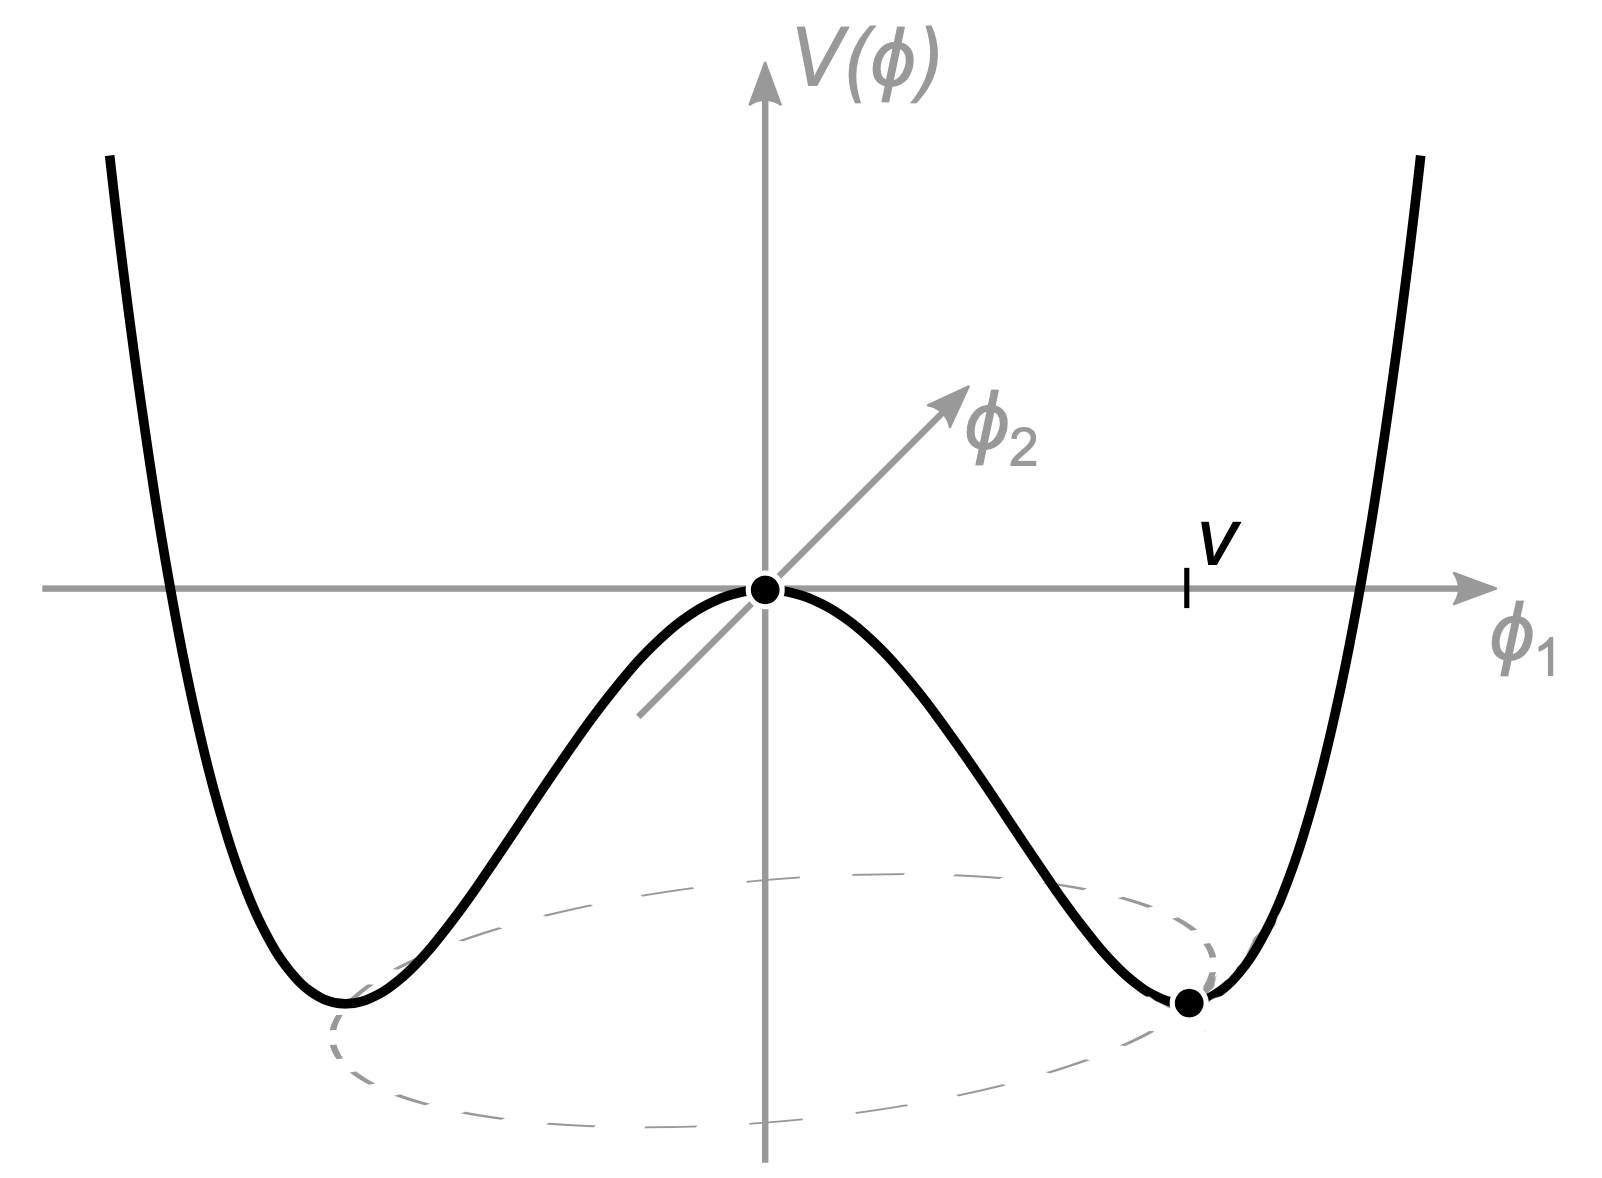
\includegraphics[width=\textwidth]{mexicanhat.png}
	\vspace{6pt}
	\caption{The Higgs potential with the two of the four field components $\phi_i$, where a rotational symmetry is implied.}
	\label{mexicanHiggs}
\end{figure}

Now let us parametrise the complex doublet field $\phi(x)$,
\be
\langle\phi\rangle=\frac{1}{\sqrt{2}}
 \begin{pmatrix}
  0 \\
  v+h(x)
 \end{pmatrix} .
 \label{higgsVparametrized}
\ee
In this case, \autoref{higgspotential} becomes,
\be
V = -\frac{1}{2}m_h^2h^2-\sqrt{\frac{\lambda}{2}}m_hh^3-\frac{1}{4}\lambda h^4 ,
\ee
where $m_h = \sqrt{2\lambda}v$. This potential describes a scalar particle. The first term represents the Higgs mass term while others represent the self interactions of Higgs.
The covariant derivative of the Higgs field is given by,
\be
  D_\mu\phi = 
  \left(\partial_\mu-ig_2A_\mu^a-i\frac{1}{2}g_1B_\mu\right)
  \phi
\ee
and now the vector bosons can be obtained from the gauge bosons as in the followings,
\be
  W_\mu^{\pm}=\frac{1}{\sqrt{2}}\left( A_\mu^1\mp A_\mu^2 \right) ,
\ee
\be
  Z_\mu=cos\theta_WA_\mu^3-sin\theta_WB_\mu ,
\ee
\be
  A_\mu=sin\theta_WA_\mu^3+cos\theta_WB_\mu ,
\ee
where
\be
  sin\theta_W = \frac{g_2}{\sqrt{g_2^2+g_1^2}} ,\; \; cos\theta_W=\frac{g_1}{\sqrt{g_2^2+g_1^2}} .
\ee
\\$\theta_W$ here is called \emph{the weak mixing angle}. Substituting \autoref{higgsVparametrized} with the kinetic term $|D_\mu\phi|^2$ in \autoref{HiggsLag} gives,
\be
\Lag_{kin}=-\frac{1}{2}\left(\partial_\mu\phi\right)^2+\left(m_W^2W^{\mu+}W_{\mu-}+\frac{1}{2}m_Z^2Z^{\mu+}Z_{\mu-}\right)\left(1+\frac{h}{v}\right)^2 ,
\ee
where the mass terms of the massive bosons such as,
\be
m_{W^\pm} = g\frac{v}{2}, \; \; m_Z = \frac{v}{2}
\ee
Leptons, similarly, acquire mass by Yukawa interactions with the Lagrangian,
\be
\Lag_{Yukawa}=-\lambda_l\psi_L\phi\psi_R
\ee
where $\lambda_l$ is the Yukawa coupling to the lepton field $\psi$. After the spontaneous symmetry breaking, the Lagrangian part of the Yukawa coupling to the leptonic field reads,
\be
\Lag_{Yukawa}=-m_f\bar ff\left(1+\frac{h}{v}\right) .
\ee
and leptons acquire mass proportional to their interactions with the Higgs field.

The Higgs boson, required for the spontaneous symmetry breaking, was found experimentally by the CMS and ATLAS experiments at the LHC Experiment at CERN\cite{HiggsCMS,HiggsATLAS} in 2012, almost 40 years after its theoretical assumption. The mass of the Higgs boson is 125 GeV and its parameters; spin, parity and branching ratios are found to be consistent with the Standard Model predictions\cite{Higgsprecision1, Higgsprecision2}.

The most general form of the SM Lagrangian depends on 19 parameters. These parameters are given in \autoref{SMparameters}.
\begin{table*}[h]
	{\setlength{\tabcolsep}{14pt}
		\caption{Parameters of the Standard Model.}
		\begin{center}
			\vspace{-6mm}
			\begin{tabular}{cccc}
				\hline \\[-2.45ex] \hline \\[-2.1ex]
				\# & Symbol & Name & Value \\
				\hline \\[-1.8ex]
				1 & $m_e$ & Electron mass & 0.511 MeV \\
				2 & $m_\mu$ & Muon mass & 105.7 MeV \\
				3 & $m_\tau$ & Tau mass & 1.78 GeV \\
				4 & $m_u$ & Up quark mass & 1.9 MeV \\
				5 & $m_d$ & Down quark mass & 4.4 MeV \\
				6 & $m_s$ & Strange quark mass & 87 MeV \\
				7 & $m_c$ & Charm quark mass & 1.32 GeV \\
				8 & $m_b$ & Bottom quark mass & 4.24 GeV \\
				9 & $m_t$ & Top quark mass & 173.5 GeV \\
				10 & $\theta_{12}$ & CKM 1-2 Mixing angle & 13.1\textdegree \\
				11 & $\theta_{23}$ & CKM 2-3 Mixing angle & 2.4\textdegree \\
				12 & $\theta_{13}$ & CKM 1-3 Mixing angle & 0.2\textdegree \\
				13 & $\delta$ & CKM CP violation Phase & 0.995 \\
				14 & $g_1$ or $g\prime$ & U(1) gauge coupling & 0.357 \\
				15 & $g_2$ or g & SU(2) gauge coupling & 0.652 \\
				16 & $g_3$ or $g_s$ & SU(3) gauge coupling & 1.221 \\
				17 & $\theta_{QCD}$ & QCD vacuum angle & $\sim $ 0 \\
				18 & $v$ & Higgs vacuum expectation value & 246 GeV \\
				19 & $m_H$ & Higgs mass & 125 GeV \\
				\hline
			\end{tabular}
			\vspace{-6mm}
		\end{center}
		\label{SMparameters}}
\end{table*}


\section{BSM Searches}

